%%%%%%%%%%%%%%%%%%%%%%%%%%%%%%%% 

\section{The Near Detector Systems Neutrino Measurements Prototyping Plan} 
\label{sec:proto-nd-nnd}


\section{The ND Beamline Measurements Prototyping Plan} 
\label{sec:proto-nd-blm}

\subsection{Prototype Development for the Cherenkov and Ionization Detectors}
\label{subsec:proto-blm-muon-cherenkov-proto}

A prototype Cherenkov counter, along with associated fully automated gas systems,
HV systems, and data acquisition system has been constructed and is undergoing
testing in the NuMI neutrino beam's muon alcove 2. In addition, three diamond
detectors~\cite{ref:CERNdiamond} for ionization measurements have also been installed into the alcove.
Figure~\ref{fig:Alcove2Cherenkov} shows the prototype detectors in NuMI alcove 2.

The counter has an automated gas system with a settable pressure that ranges
from vacuum to 20 atm, corresponding to muon Cherenkov thresholds of 
200 GeV/c and 1 GeV/c respectively. When operated at vacuum, the PMT registers all background light
unrelated to the gas, e.g. transition radiation, light from particles hitting the window and PMT glass.
Those contributions are observed to be very small relative to the coherent, directional Cherenkov light.

The counter is constructed with a 1 meter long radiator section
as shown in Figure~\ref{fig:CherenkovCounterDetail} . A 20 foot extension allows the reflected 
Cherenkov light to travel to a sapphire pressure window viewed by a photo multiplier tube.

The prototype is now fully integrated into NuMI operations and real-time waveforms can be viewed online as shown in Figure~\ref{fig:MuonDetectorWaveforms}. The top panel shows the waveform from the Cherenkov counter at 2 atm gas pressure, that corresponds to a muon momentum threshold of 3 GeV/c. The second panel shows the waveform from a $9mm\ \times\ 9mm$ diamond detector mounted to the front flange of the Cherenkov radiator section as shown in the inset 
of Figure~\ref{fig:Alcove2Cherenkov}.

The extracted NuMI proton beam, Resistive Wall Monitor (RWM) signal 
is also recorded with an identical digitizer. That allows a direct, bucket-by-bucket (individual proton pulses) 
comparison of the proton current onto the NuMI primary proton target, and the muons measured after the absorber with a 400ps time resolution.

\begin{cdrfigure}[Muon gas Cherenkov counter]{Alcove2Cherenkov}{A prototype muon gas Cherenkov detector for DUNE.  
Muons travel through an L-shaped 4" Conflat pipe filled with a pressurized gas. A flat mirror mirrors directs the optical photons to a photo multiplier. The lower right inset shows the 20 bar MKS pressure reading achieved by the Cherenkov gas system, and the inset on the upper right shows the CERN/Cividec diamond detectors mounted to the Cherenkov housing.}
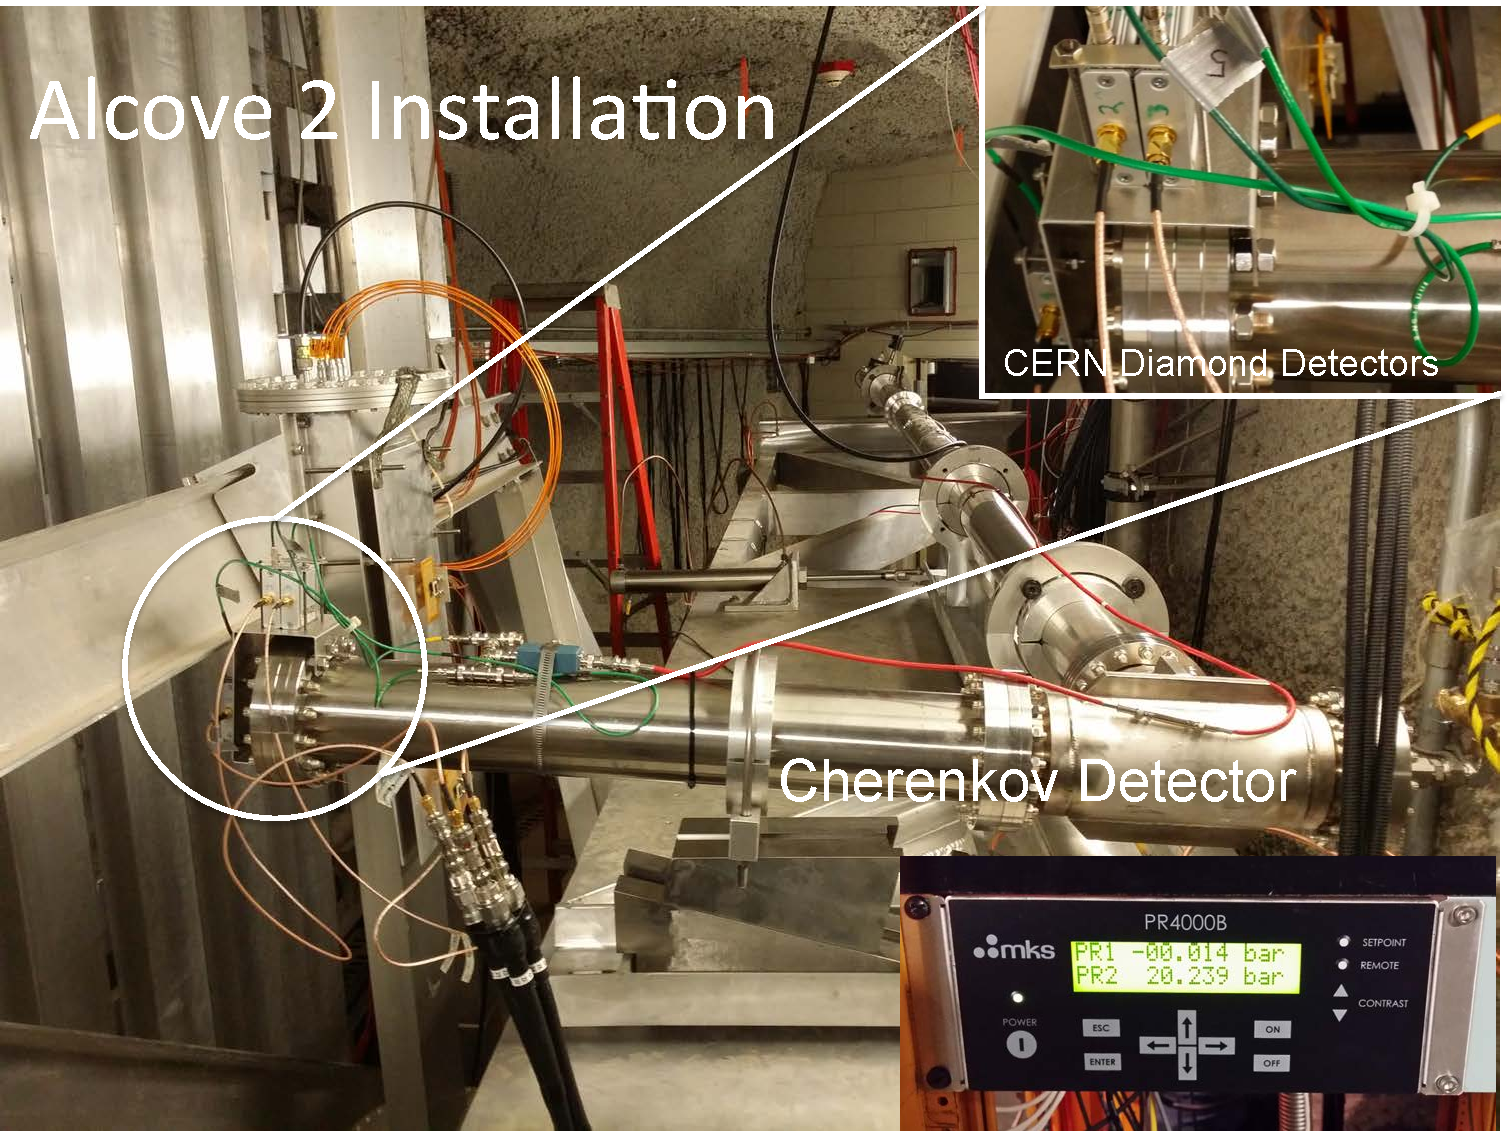
\includegraphics[width=5.5in]{Alcove2Cherenkov}
\end{cdrfigure}

\begin{cdrfigure}[Muon Detector Waveforms]{MuonDetectorWaveforms}{The realtime display of the
muon detector prototypes in operation on the NuMI beam line. The top two panels are the Cherenkov counter and CERN diamond detector \cite{ref:CERNdiamond}, The signals are transmitted through low-loss heliax cable, and then the waveform is digitized at 2.5 GHz with a 12 bit dynamic range, and the recorded onto disk storage for analysis. The signal from the muons is contained in the short beam pulse "buckets" created by the accelerator RF structure. The fast timing allows the prompt muon signal to be easily separated from potential backgrounds such as stopped muon decays, beta decays, and neutrons.}
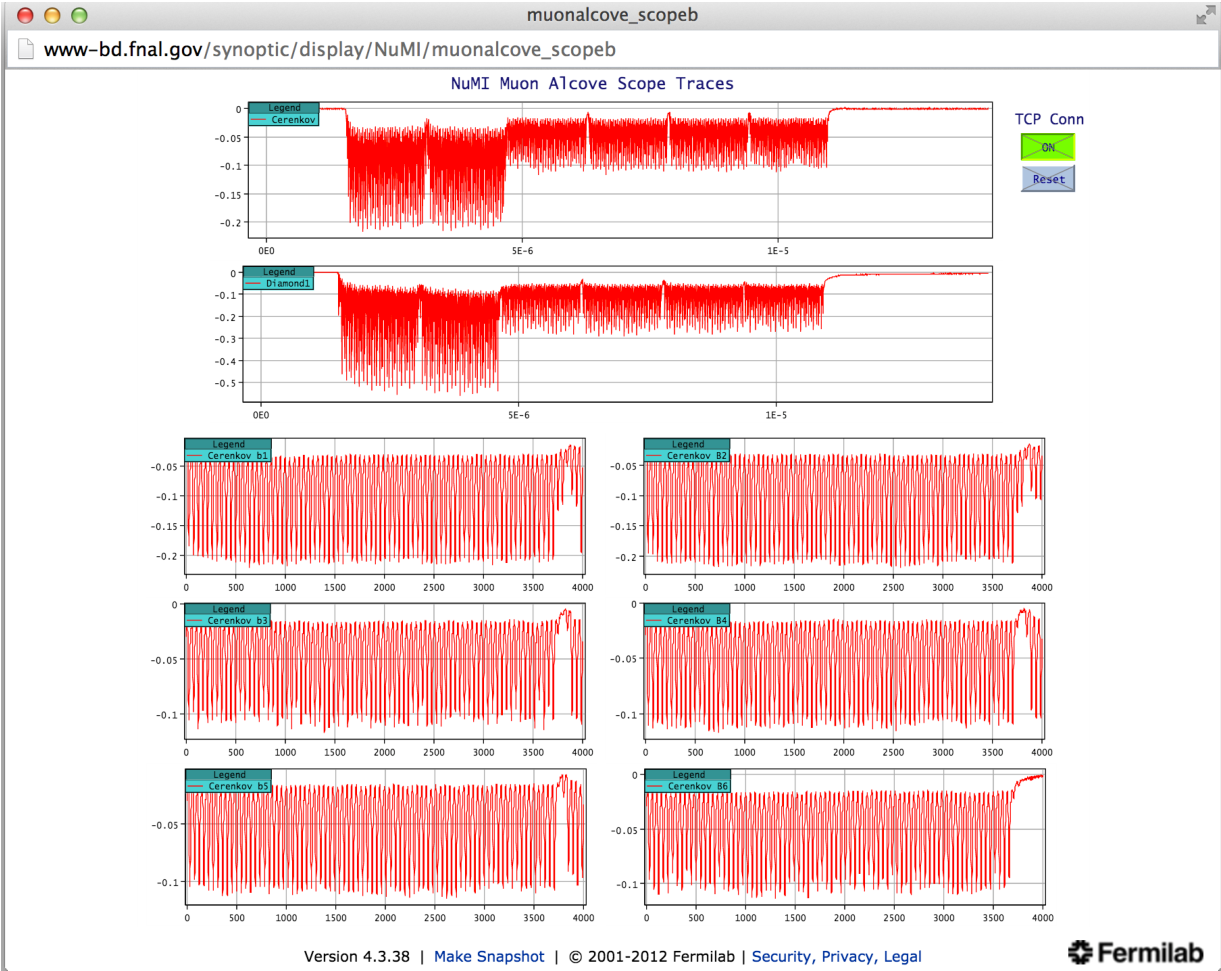
\includegraphics[width=5in]{MuonDetectorWaveforms}
\end{cdrfigure}

\subsubsection{Prototype Development of the Stopped Muon Counters}

Prototype development activity for the Michel-electron detectors will
be divided into studies of the rate and radiation environment where
the detectors will be located and development of the counters
themselves. 

The radiation environment will be studied both with Monte Carlo 
simulations and by measurements from initial prototype detectors 
in the NuMI muon alcoves \cite{ref:NuMIBeamMonitors}.
The prototypes will be installed into the alcoves in 2016 and 2017.
Studies will be performed to determine if the photon sensors
can survive the radiation environment at the location of the Michel
detector. If the sensors can survive, they can be attached directly to
the Cherenkov medium; if not, optical guides will have to bring the
light to a lower-radiation area to the side of the beam. Potential
radiation damage to the Cherenkov radiator itself will also be
studied.

The detector design will focus on selecting radiator and shielding
material, photon-detection technology and control/readout
hardware. Possible radiators include aerogel, which may be designed to
be replaced periodically, and flowing liquids such as H$_2$O or
mineral oil. Long-timescale saturation from the very high-rate
environment of the beam spill could affect the photon-counting devices
\cite{ref:HighRateCounting}. Thus, it will likely be necessary to
design fast-switching, high-voltage circuits that turn on the photon
counters in the first few microseconds after the spill is over. A
similar system was developed in the 1990s for the Brookhaven Muon
(g-2) Experiment~\cite{ref:G2} .

\subsection{Current Prototyping Activities}

A second set of muon detectors, the final DUNE design, are being constructed at this time (2015). They are being installed directly behind the NuMI proton beam dump (muon alcove 1). The detectors will be mounted on a movable stand which has undergone an engineering review at Fermilab. The entire setup, detectors and stand, will be suitable for use in the DUNE beam.

The entire setup will be eventually transferred the DUNE absorber hall. The higher radiation environment of alcove 1 will be more similar to the eventual DUNE installation. It will allow the DUNE muon detectors to be calibrated in the NuMI beam and ready for use in the DUNE beam.

